\mode*
\lecture[tcp]{TCP}{tcp}
%\mode<article>{\clearpage}
\section{Transport Protocols}

\paragraph{Why need transport layer?}

  Why need transport layer if its service is so similar to the network layer service? The
  answer is subtle, but crucial. \emph{The transport code runs entirely on the users' machines,
  but the network layer mostly runs on the routers, which are operated by the carrier} (at
  least for a wide area network). \citetitle[Sec.~6.1.1, \emph{Services provided to the upper
    layers}]{tanenbaum2011computer}
  \begin{itemize}
  \item What happens if the network layer offers inadequate service?
  \item What if it frequently loses packets?
  \item What happens if routers crash from time to time?
  \end{itemize}
  Problems occur, that's what. \emph{The users have no real control over the network layer}, so
  they cannot solve the problem of poor service by using better routers or putting more
  error handling in the data link layer because they don't own the routers. The only
  possibility is to put on top of the network layer another layer that improves the
  quality of the service.

  \emph{If all real networks were flawless and all had the same service primitives and
    were guaranteed never, ever to change, the transport layer might not be needed.}

\begin{frame}{\scalebox{1.5}{🕿}\quad vs.\quad\scalebox{1.5}{🖃}}
  \begin{minipage}[t]{.47\linewidth}
    \begin{iblock}{Circuit switching (🕿)}
      \begin{itemize}
      \item[🙂] guaranteed performance
      \item[🙂] fast transfers (once circuit is established)
      \item[\alert{🙁}] wastes bandwidth if traffic is ``bursty''
      \item[\alert{🙁}] connection setup adds delay
      \item[\alert{🙁}] recovery from failure is slow
      \end{itemize}
    \end{iblock}
  \end{minipage}\hfill
  \begin{minipage}[t]{.47\linewidth}
    \begin{iblock}{Packet switching (🖃)}
      \begin{itemize}
      \item[\alert{🙁}] no guaranteed performance
      \item[\alert{🙁}] header overhead per packet
      \item[\alert{🙁}] queues and queuing delay
      \item[🙂] efficient use of bandwidth
      \item[🙂] no connection setup
      \item[🙂] can ``route around trouble''
      \end{itemize}
    \end{iblock}
  \end{minipage}
\end{frame}

See also:
\begin{itemize}
\item \citetitle[Sec.~1.3.3, \emph{Connection-Oriented Versus Connectionless
    Service}]{tanenbaum2011computer}
\item \citetitle[Sec.~4.2, \emph{Virtual Circuit and Datagram Networks}]{kurose2013computer}
\item
  \url{http://courses.iddl.vt.edu/CS1604/15-Lesson_14/04-Connection-Oriented_vs_Connectionless.php}
\item \url{http://www.cisco.com/cpress/cc/td/cpress/fund/ith2nd/it2401.htm#xtocid1500020}
\item
  \url{http://www.inetdaemon.com/tutorials/basic_concepts/communication/connection-oriented_vs_connectionless.shtml}
\item \url{http://www.cs.virginia.edu/~zaher/classes/CS457/lectures/network_1.pdf}
\end{itemize}

\subsection{TCP}

\begin{frame}
  \begin{iblock}{}
    \begin{minipage}{.5\linewidth}
      \begin{description}
      \item[IP:] host {\Large {\dejavu ↔}} host
      \item[TCP/UDP:] process {\Large {\dejavu ↔}} process
      \end{description}
    \end{minipage}\hfill
    \begin{minipage}{.5\linewidth}
      \begin{center}
        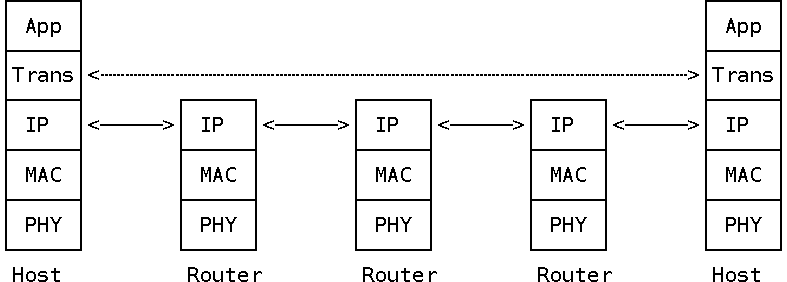
\includegraphics[width=\linewidth]{host2host}
      \end{center}
    \end{minipage}
  \end{iblock}
  \begin{minipage}[t]{.5\linewidth}
    \begin{iblock}{IP: Best-effort, no guarantee}
      \begin{itemize}
      \item[?] segment delivery
      \item[?] orderly delivery of segments
      \item[?] the integrity of the data in the segments
      \end{itemize}
    \end{iblock}
  \begin{iblock}{QoS on data link layer or IP layer?}
    \begin{itemize}
    \item[\alert{🙁}] Efficiency
    \item[\alert{🙁}] Upgrade all the routers
    \end{itemize}
  \end{iblock}
\end{minipage}\hfill
  \begin{minipage}[t]{.5\linewidth}
    \begin{iblock}{TCP: Receive it correctly and orderly or none}
      \begin{itemize}
      \item[✔] correctness --- acknowledgement, checksum
      \item[✔] order --- sequence numbers
      \item[✔] packet lost --- timers
      \item[✔] flow control --- sliding window
      \item[✔] congestion control
      \end{itemize}
    \end{iblock}
  \end{minipage}
    % \begin{tikzpicture}[remember picture, overlay]
  %     \node [red,opacity=.4,anchor=north east, scale=.5] at (current page.north east)%
  %     {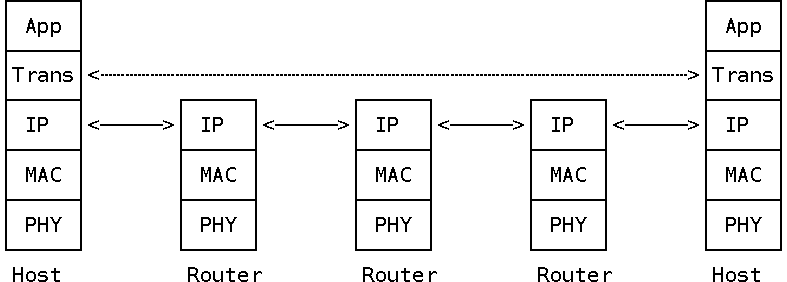
\includegraphics{host2host}};    
  % \end{tikzpicture}
\end{frame}

\begin{description}
\item[Why doesn't IP provides reliable service?]\,
  \begin{itemize}
  \item Inefficient. Routers are very busy forwarding data packets as fast as possible. It
    would be slow down upon providing extra functionalities.
  \item Unnecessary. The end process has to check the received data for correctness and
    orderliness anyway even if each router provides guaranteed delivery service.
  \end{itemize}
\item[TCP is optimized for accurate delivery rather than timely delivery] TCP sometimes
  incurs relatively long delays (on the order of seconds) while waiting for out-of-order
  messages or retransmissions of lost messages. It is not particularly suitable for
  real-time applications such as Voice over IP. For such applications, protocols like the
  Real-time Transport Protocol (RTP) running over the User Datagram Protocol (UDP) are
  usually recommended instead\citetitle[Sec.~2, \emph{Network Function}]{wiki:tcp}.
\end{description}

From \url{http://ssfnet.org/Exchange/tcp/tcpTutorialNotes.html}:
\begin{description}
\item[Stream Data Transfer] From the application's viewpoint, TCP transfers a contiguous
  stream of bytes. TCP does this by grouping the bytes in TCP segments, which are passed
  to IP for transmission to the destination. TCP itself decides how to segment the data
  and it may forward the data at its own convenience.
\item[Reliability] TCP assigns a sequence number to each byte transmitted, and expects a
  positive acknowledgment (ACK) from the receiving TCP. If the ACK is not received within
  a timeout interval, the data is retransmitted. The receiving TCP uses the sequence
  numbers to rearrange the segments when they arrive out of order, and to eliminate
  duplicate segments.
\item[Flow Control] The receiving TCP, when sending an ACK back to the sender, also
  indicates to the sender the number of bytes it can receive beyond the last received TCP
  segment, without causing overrun and overflow in its internal buffers. This is sent in
  the ACK in the form of the highest sequence number it can receive without problems.
\item[Multiplexing] To allow for many processes within a single host to use TCP
  communication facilities simultaneously, the TCP provides a set of addresses or ports
  within each host. Concatenated with the network and host addresses from the internet
  communication layer, this forms a socket. A pair of sockets uniquely identifies each
  connection.
\item[Logical Connections] The reliability and flow control mechanisms described above
  require that TCP initializes and maintains certain status information for each data
  stream. The combination of this status, including sockets, sequence numbers and window
  sizes, is called a logical connection. Each connection is uniquely identified by the
  pair of sockets used by the sending and receiving processes.
\item[Full Duplex] TCP provides for concurrent data streams in both directions.
\item[TCP provides a connection over a connectionless IP layer] A connection, likes a water
  pipe, has:
  \begin{itemize}
  \item two ends
  \item a stream flowing in it sequentially
  \item flow control mechanisms
  \end{itemize}

  The reliability and flow control mechanisms described above require that TCPs initialize
  and maintain certain status information for each data stream.  The combination of this
  information, including sockets, sequence numbers, and window sizes, is called \emph{a
    connection}.  Each connection is uniquely specified by a pair of sockets identifying
  its two sides\citetitle[Sec 1.5, \emph{RFC 793}]{rfc793}.
\end{description}

\begin{frame}{A TCP Connection Over A Connectionless IP Layer}
  \CMD{ss -4t state established}
  \begin{center}\ttfamily
    \begin{tblr}{colspec={@{}lllll@{}},row{1}={gray9,font=\bfseries}}
      Recv-Q& Send-Q& Local Address:Port && Peer Address:Port \\    
      0     & 0     &     127.0.0.1:3333 &&    127.0.0.1:14624\\
      0     & 0     &     127.0.0.1:14624&&    127.0.0.1:3333 \\\cline{3-3}\cline{5-5}
      &&\SetCell{c}\textbf{Socket}&&\SetCell{c}\textbf{Socket}\\\cline{3-5}
      &&\SetCell[c=3]{c}\textbf{Connection}\\
    \end{tblr}
  \end{center}
  \begin{iblock}{Port numbers}
    \begin{description}
    \item[port range:] 0 \char`~{} 65535
    \item[well-known ports:] 0 \char`~{} 1023
    \end{description}
    \begin{center}
      \begin{tblr}{colspec={rl|rl|rl},rowsep=0pt}
        FTP &20/21&SSH&22&Telnet&23\\
        SMTP&25 &DNS&53&DHCP &67/68\\
        HTTP&80 &POP3&110&HTTPS&443\\
        IMAP4&143&&&&
      \end{tblr}
    \end{center}
  \end{iblock}
\end{frame}

\begin{frame}{TCP Header}
  \centering
  \mode<beamer>{ 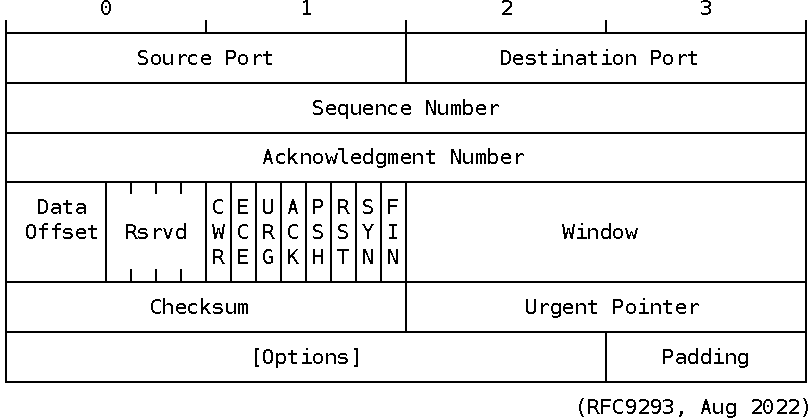
\includegraphics[width=\textwidth]{tcp-hdr} }%
  \mode<article>{ 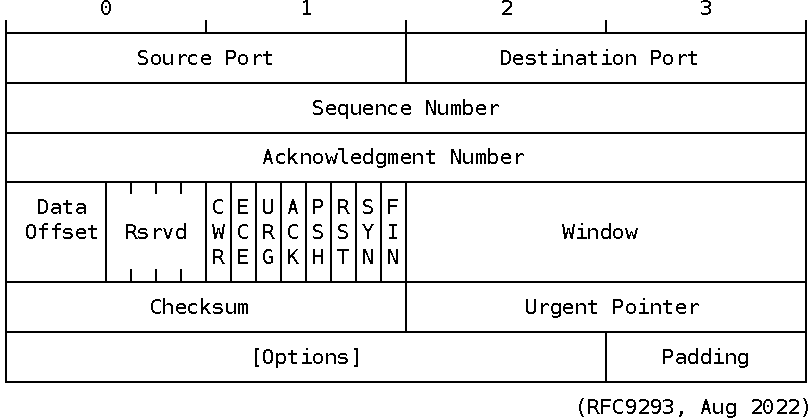
\includegraphics[width=.6\textwidth]{tcp-hdr}\label{fig:tcp-segment-format} }
\end{frame}

See also\citetitle[Sec.~3, \emph{TCP Segment Structure}]{wiki:tcp}.
\begin{description}
\item[Source port (16 bits)] identifies the sending port
\item[Destination port (16 bits)] identifies the receiving port
\item[Sequence number (32 bits)] has a dual role:
  \begin{itemize}
  \item If the SYN flag is set (1), then this is the initial sequence number. The sequence
    number of the actual first data byte and the acknowledged number in the corresponding
    ACK are then this sequence number plus 1.
  \item If the SYN flag is clear (0), then this is the accumulated sequence number of the
    first data byte of this segment for the current session.
  \end{itemize}
  Sequence numbers allow receivers to discard duplicate packets and properly sequence
  reordered packets.
\item[Acknowledgment number (32 bits)] if the ACK flag is set then the value of this field
  is the next sequence number that the receiver is expecting. This acknowledges receipt of
  all prior bytes (if any). The first ACK sent by each end acknowledges the other end's
  initial sequence number itself, but no data.

  Acknowledgments allow senders to determine when to retransmit lost packets.
\item[Data offset (4 bits)] specifies the size of the TCP header in 32-bit words. The
  minimum size header is 5 words and the maximum is 15 words thus giving the minimum size
  of 20 bytes and maximum of 60 bytes, allowing for up to 40 bytes of options in the
  header. This field gets its name from the fact that it is also the offset from the start
  of the TCP segment to the actual data.
\item[Reserved (3 bits)] for future use and should be set to zero
\item[Flags (9 bits) (aka Control bits)] contains 9 1-bit flags
  \begin{itemize}
  \item NS (1 bit) – ECN-nonce concealment protection (experimental: see RFC 3540).
  \item CWR (1 bit) – Congestion Window Reduced (CWR) flag is set by the sending host to
    indicate that it received a TCP segment with the ECE flag set and had responded in
    congestion control mechanism (added to header by RFC 3168).
  \item ECE (1 bit) – ECN-Echo has a dual role, depending on the value of the SYN flag. It
    indicates:
    \begin{itemize}
    \item If the SYN flag is set (1), that the TCP peer is ECN capable.
    \item If the SYN flag is clear (0), that a packet with Congestion Experienced flag in
      IP header set is received during normal transmission (added to header by RFC 3168).
    \end{itemize}
  \item URG (1 bit) – indicates that the Urgent pointer field is significant
  \item ACK (1 bit) – indicates that the Acknowledgment field is significant. All packets
    after the initial SYN packet sent by the client should have this flag set.
  \item PSH (1 bit) – Push function. Asks to push the buffered data to the receiving
    application. (See \citetitle[Sec.~4.2.2.2, \emph{RFC 1122}]{rfc1122} for more details)
  \item RST (1 bit) – Reset the connection
  \item SYN (1 bit) – Synchronize sequence numbers. Only the first packet sent from each
    end should have this flag set. Some other flags and fields change meaning based on
    this flag, and some are only valid for when it is set, and others when it is clear.
  \item FIN (1 bit) – No more data from sender
  \end{itemize}
\item[Window size (16 bits)] the size of the receive window, which specifies the number of
  window size units (by default, bytes) (beyond the sequence number in the acknowledgment
  field) that the sender of this segment is currently willing to receive (see also
  \citetitle[Sec.~4.4.3, \emph{Flow control}]{wiki:tcp} and \citetitle[Sec.~4.7, \emph{Window
    Scaling}]{wiki:tcp})
\item[Checksum (16 bits)] The 16-bit checksum field is used for error-checking of the
  header and data
\item[Urgent pointer (16 bits)] if the URG flag is set, then this 16-bit field is an
  offset from the sequence number indicating the last urgent data byte
\item[Options (Variable 0–320 bits, divisible by 32)] The length of this field is
  determined by the data offset field. Options have up to three fields: Option-Kind (1
  byte), Option-Length (1 byte), Option-Data (variable). The Option-Kind field indicates
  the type of option, and is the only field that is not optional. Depending on what kind
  of option we are dealing with, the next two fields may be set: the Option-Length field
  indicates the total length of the option, and the Option-Data field contains the value
  of the option, if applicable. For example, an Option-Kind byte of \texttt{0x01}
  indicates that this is a No-Op option used only for padding, and does not have an
  Option-Length or Option-Data byte following it. An Option-Kind byte of 0 is the End Of
  Options option, and is also only one byte. An Option-Kind byte of \texttt{0x02} indicates that
  this is the Maximum Segment Size option, and will be followed by a byte specifying the
  length of the MSS field (should be \texttt{0x04}). Note that this length is the total length of
  the given options field, including Option-Kind and Option-Length bytes. So while the MSS
  value is typically expressed in two bytes, the length of the field will be 4 bytes (+2
  bytes of kind and length). In short, an MSS option field with a value of \texttt{0x05B4} will
  show up as (\texttt{0x02 0x04 0x05B4}) in the TCP options section.
    
  Some options may only be sent when SYN is set; they are indicated below as
  [SYN]. Option-Kind and standard lengths given as (Option-Kind,Option-Length).
  \begin{itemize}
  \item 0 (8 bits) – End of options list
  \item 1 (8 bits) – No operation (NOP, Padding) This may be used to align option fields
    on 32-bit boundaries for better performance.
  \item 2,4,SS (32 bits) – Maximum segment size (see maximum segment size) [SYN]
  \item 3,3,S (24 bits) – Window scale (see window scaling for details)
    [SYN]\citetitle[Sec.~2.2, \emph{RFC 1323}]{rfc1323}
  \item 4,2 (16 bits) – Selective Acknowledgement permitted. [SYN] (See selective
    acknowledgments for details)\citetitle[Sec.~2, \emph{RFC 2018}]{rfc2018}
  \item 5,N,BBBB,EEEE,... (variable bits, N is either 10, 18, 26, or 34)- Selective
    ACKnowledgement (SACK)\citetitle[Sec.~3,\emph{RFC 2018}]{rfc2018} These first two bytes are
    followed by a list of 1–4 blocks being selectively acknowledged, specified as 32-bit
    begin/end pointers.
  \item 8,10,TTTT,EEEE (80 bits)- Timestamp and echo of previous timestamp (see TCP
    timestamps for details)\citetitle[Sec.~3.2,\emph{RFC 1323}]{rfc1323}
  \item[] (The remaining options are historical, obsolete, experimental, not yet
    standardized, or unassigned)
  \end{itemize}
\item[Padding] The TCP header padding is used to ensure that the TCP header ends and data
  begins on a 32 bit boundary. The padding is composed of zeros.\citetitle[Sec.~3.1, \emph{RFC
    793}]{rfc793}
\end{description}

See also: \citetitle{rfc879, rfc6691}

\paragraph{Difference between push and urgent}

\begin{itemize}
\item \url{https://stackoverflow.com/questions/9153566/difference-between-push-and-urgent-flags-in-tcp}
\end{itemize}

They are two vastly different mechanisms.
\begin{description}
\item[PSH and the PUSH function] When you send data, your TCP buffers it. So if you send a
  character it won't send it immediately but wait to see if you've got more. But maybe you
  want it to go straight on the wire: this is where the PUSH function comes in. If you
  PUSH data your TCP will immediately create a segment (or a few segments) and push them.

  But the story doesn't stop here. When the peer TCP receives the data, it will naturally
  buffer them \emph{it won't disturb the application for each and every byte}. Here's
  where the PSH flag kicks in. If a receiving TCP sees the PSH flag it will immediately
  push the data to the application.

  There's no API to set the PSH flag. Typically it is set by the kernel when it empties
  the buffer. From TCP/IP Illustrated\citetitle[Sec.~20.5 \emph{PUSH Flag}]{fall2011tcp}:

\begin{quote}
  This flag is conventionally used to indicate that the buffer at the side sending the
  packet has been emptied in conjunction with sending the packet. In other words, when the
  packet with the PSH bit field set left the sender, the sender had no more data to send.
\end{quote}

But be aware Stevens also says:

\begin{quote}
  Push (the receiver should pass this data to the application as soon as possible—not
  reliably implemented or used)
\end{quote}

\item[URG and OOB data] TCP is a stream-oriented protocol. So if you push 64K bytes on one
  side, you'll eventually get 64k bytes on the other. So imagine you push a lot of data
  and then have some message that says ``Hey, you know all that data I just sent ? Yeah,
  throw that away''. The gist of the matter is that once you push data on a connection you
  have to wait for the receiver to get all of it before it gets to the new data.

  This is where the URG flag kicks in. When you send urgent data, your TCP creates a
  special segment in which it sets the URG flag and also the urgent pointer field. This
  causes the receiving TCP to forward the urgent data on a separate channel to the
  application (for instance on Unix your process gets a SIGURG). This allows the
  application to process the data \emph{out of band}.

\begin{quote}
  RFC 6093 disagrees with this use of ``out of band'' and states\citetitle[\emph{RFC
    6093}]{rfc6093}:

  The TCP urgent mechanism is NOT a mechanism for sending ``out-of-band'' data: the
  so-called ``urgent data'' should be delivered ``in-line'' to the TCP user.

  But then it goes on to admit:

  By default, the last byte of ``urgent data'' is delivered ``out of band'' to the
  application. That is, it is not delivered as part of the normal data stream.

  An application has to go out of its way and specify e.g. \texttt{SO\_OOBINLINE} to get
  standards-conforming urgent semantics.

  If all this sounds complicated just \emph{don't use urgent data}.
\end{quote}

As a side note, it's important to be aware that urgent data is rarely used today and not
very well implemented. It's far easier to use a separate channel or a different approach
altogether.
\end{description}

\begin{frame}{Establishing a TCP Connection}
  \begin{center}
    \mode<beamer>{ 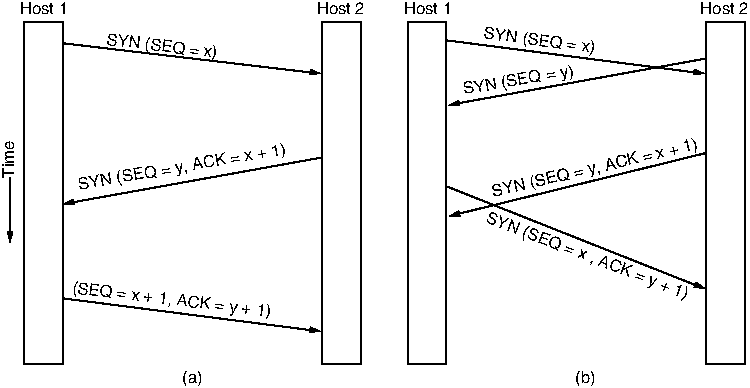
\includegraphics[width=\textwidth]{3way} }%
    \mode<article>{ 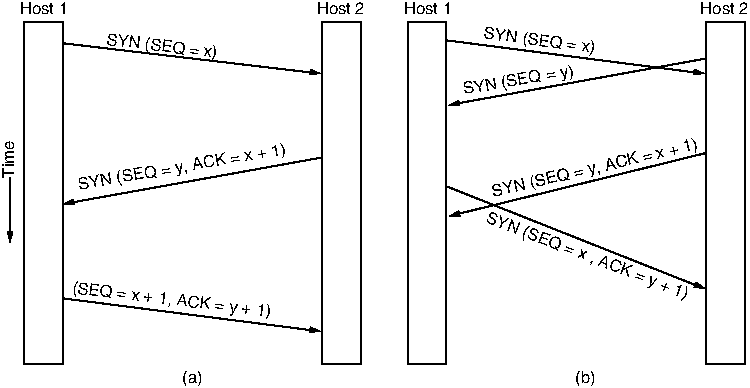
\includegraphics[width=.6\textwidth]{3way} }
  \end{center}
  \label{fig:3way}
\end{frame}

To establish a connection, TCP uses a three-way handshake. Before a client attempts to
connect with a server, the server must first bind to and listen at a port to open it up
for connections: this is called a passive open. Once the passive open is established, a
client may initiate an active open. To establish a connection, the three-way (or 3-step)
handshake occurs \citetitle[Sec.~4.1, \emph{Connection establishment}]{wiki:tcp}:
\begin{enumerate}
\item \texttt{SYN}: The active open is performed by the client sending a \texttt{SYN} to
  the server. The client sets the segment's sequence number to a random value \texttt{A}.
\item \texttt{SYN-ACK}: In response, the server replies with a \texttt{SYN-ACK}. The
  acknowledgment number is set to one more than the received sequence number
  i.e. \texttt{A+1}, and the sequence number that the server chooses for the packet is
  another random number, \texttt{B}.
\item \texttt{ACK}: Finally, the client sends an \texttt{ACK} back to the server. The
  sequence number is set to the received acknowledgement value i.e. \texttt{A+1}, and the
  acknowledgement number is set to one more than the received sequence number
  i.e. \texttt{B+1}.
\end{enumerate}

At this point, both the client and server have received an acknowledgment of the
connection. The steps 1, 2 establish the connection parameter (sequence number) for one
direction and it is acknowledged. The steps 2, 3 establish the connection parameter
(sequence number) for the other direction and it is acknowledged. With these, a
full-duplex communication is established.

\begin{itemize}
\item See also \citetitle[Sec.~6.2.2 \emph{Connection Establishment}; Sec.~6.5.5, \emph{TCP
    Connection Establishment}]{tanenbaum2011computer}.
\item More about Initial Sequence Number (ISN) see
  \citetitle[Sec.~13.2.3 \emph{Initial Sequence Number (ISN)}]{fall2011tcp}.
\end{itemize}

\begin{frame}{Closing a TCP Connection}
  \begin{center}
    \mode<beamer>{ 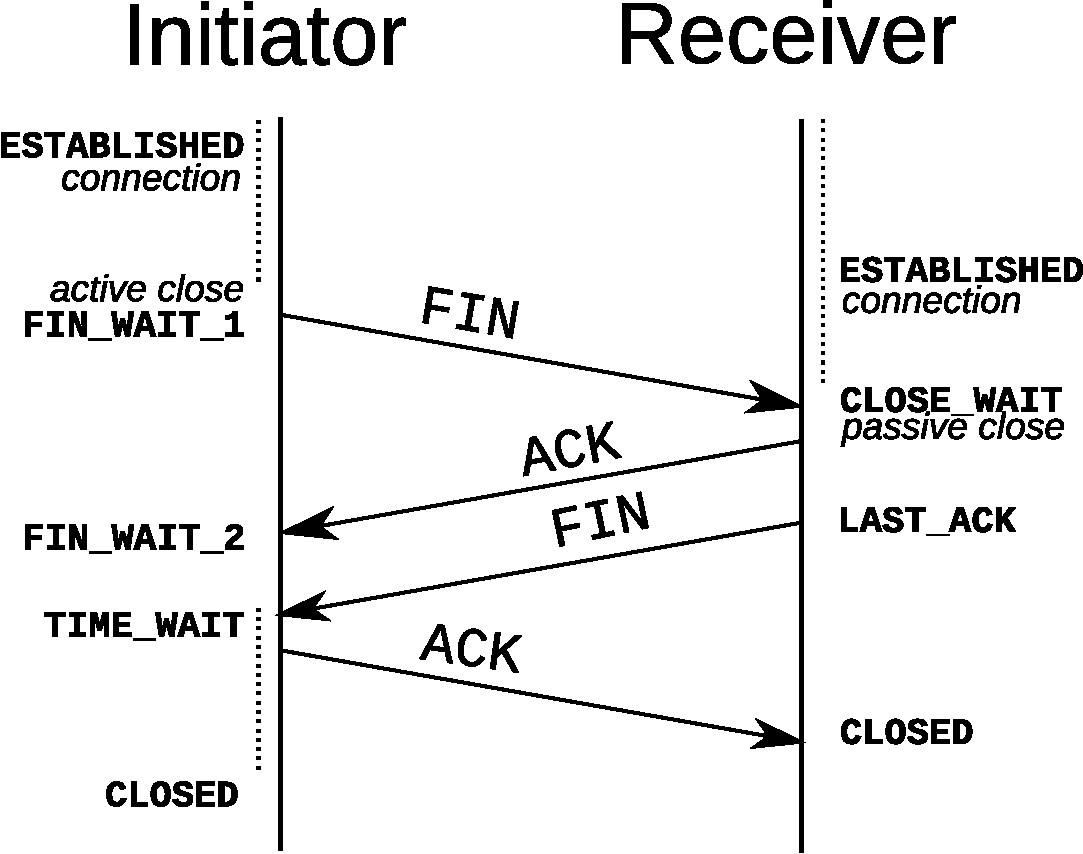
\includegraphics[width=.7\textwidth]{3way-close} }%
    \mode<article>{ 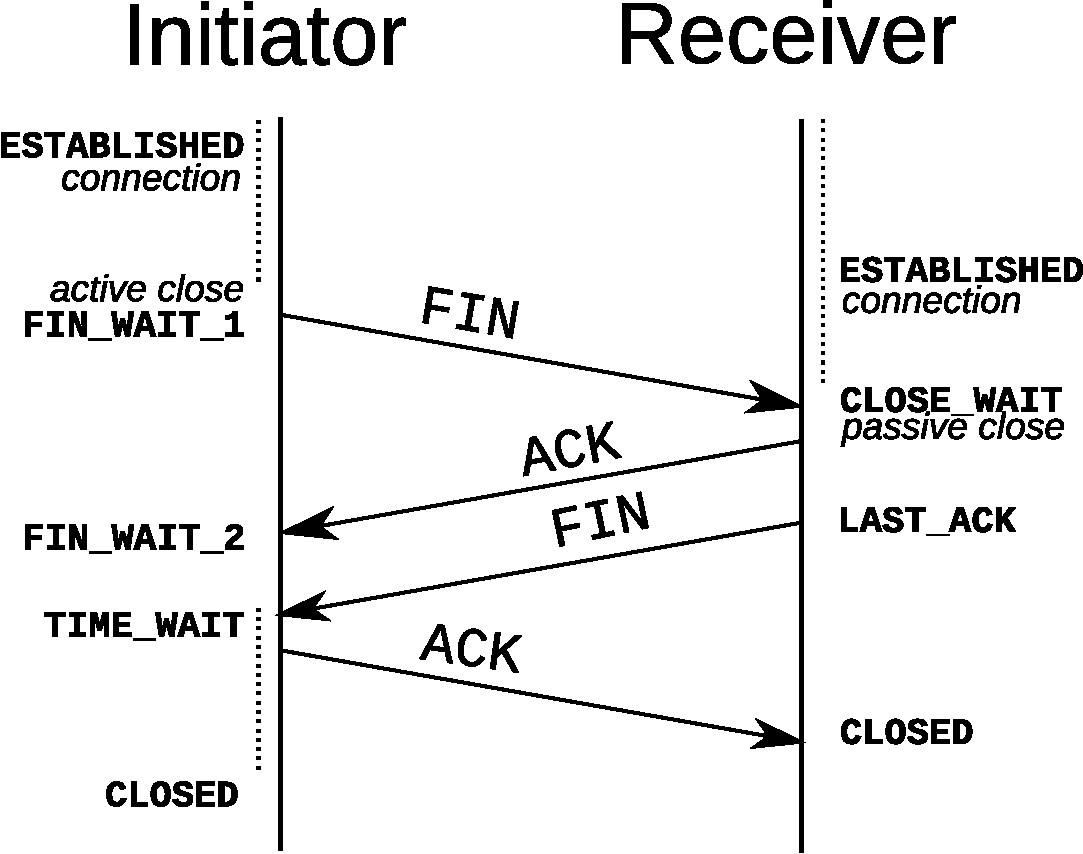
\includegraphics[width=.3\textwidth]{3way-close} }
  \end{center}
  \label{fig:3way-close}
\end{frame}

The connection termination phase uses a four-way handshake, with each side of the
connection terminating independently. When an endpoint wishes to stop its half of the
connection, it transmits a FIN packet, which the other end acknowledges with an
ACK. Therefore, a typical tear-down requires a pair of FIN and ACK segments from each TCP
endpoint. After both FIN/ACK exchanges are concluded, the side that sent the first FIN
before receiving one waits for a timeout before finally closing the connection, during
which time the local port is unavailable for new connections; this prevents confusion due
to delayed packets being delivered during subsequent connections. \citetitle[Sec.~4.2,
\emph{Connection termination}]{wiki:tcp}

A connection can be ``half-open'', in which case one side has terminated its end, but the
other has not. The side that has terminated can no longer send any data into the
connection, but the other side can. The terminating side should continue reading the data
until the other side terminates as well.

It is also possible to terminate the connection by a 3-way handshake, when host A sends a
FIN and host B replies with a FIN \& ACK (merely combines 2 steps into one) and host A
replies with an ACK. This is perhaps the most common method.

Some host TCP stacks may implement a half-duplex close sequence, as Linux or HP-UX do. If
such a host actively closes a connection but still has not read all the incoming data the
stack already received from the link, this host sends a RST instead of a FIN (Section
4.2.2.13 in \citetitle[\emph{RFC 1122}]{rfc1122}). This allows a TCP application to be sure the
remote application has read all the data the former sent—waiting the FIN from the remote
side, when it actively closes the connection. But the remote TCP stack cannot distinguish
between a Connection Aborting RST and Data Loss RST. Both cause the remote stack to lose
all the data received.

\begin{frame}%{Three-way Handshake}
  \begin{minipage}{.78\linewidth}
    \begin{description}
    \item[Terminal A:] \texttt{nc -l 3333}
    \item[Terminal B:] \texttt{nc localhost 3333}
    \item[Terminal C:] \texttt{sudo tcpdump -i lo -S port 3333}
    \end{description}
  \end{minipage}\hfill
  \begin{minipage}{.2\linewidth}
    \includegraphics[width=\textwidth]{3333}
  \end{minipage}
  \begin{center}
    \mode<beamer>{ \includegraphics[width=.9\textwidth]{tcpdump} }%
    \mode<article>{ \includegraphics[width=.7\textwidth]{tcpdump} }
  \end{center}
\end{frame}

\begin{frame}<beamer>
  \centering
  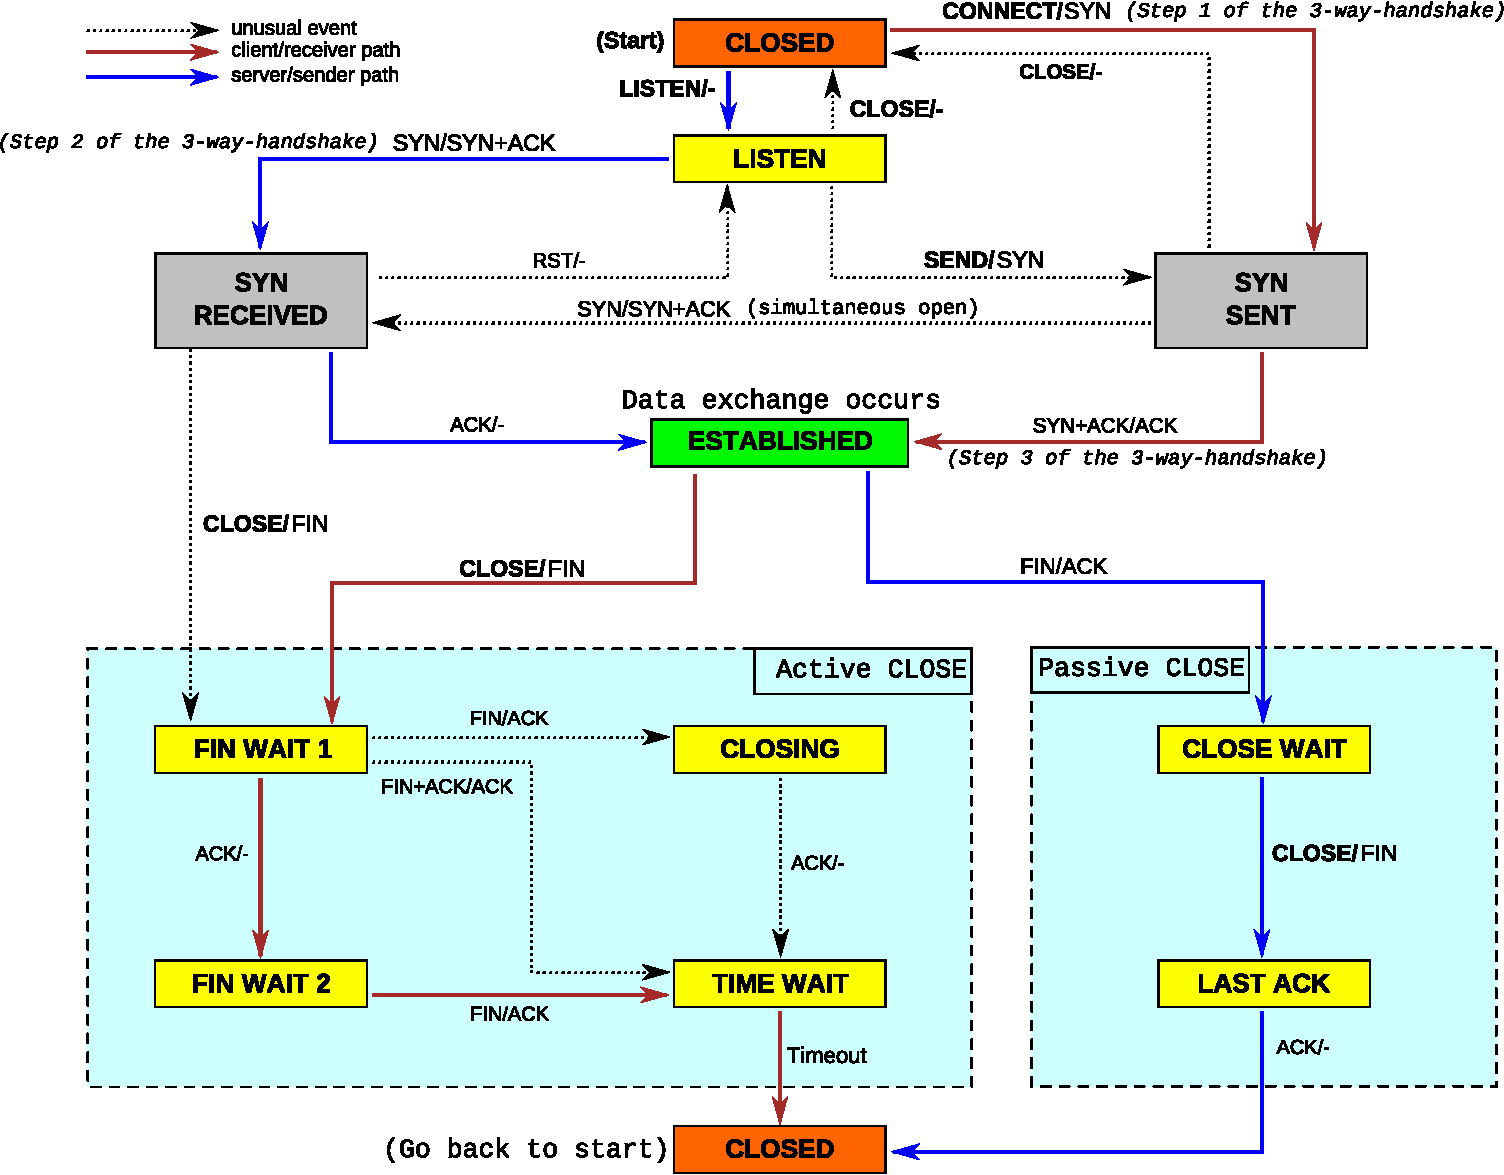
\includegraphics[height=\textheight]{state-wikipedia}
\end{frame}

\begin{figure}[!ht]
  \centering
  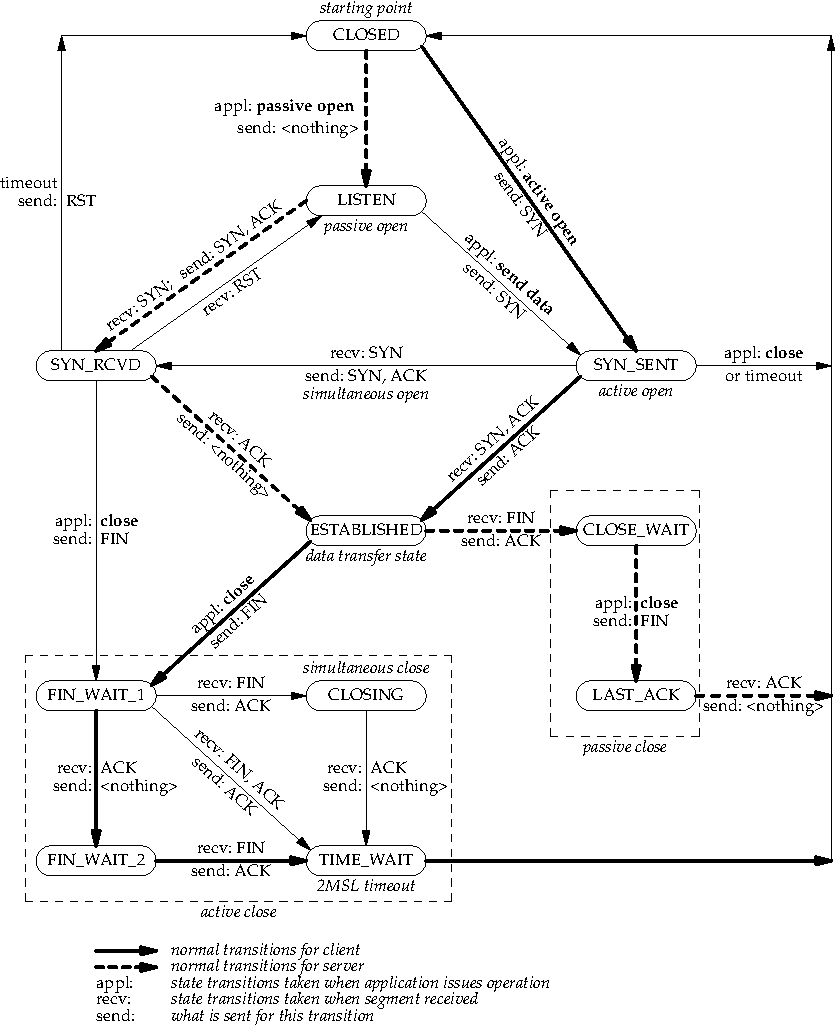
\includegraphics[width=\textwidth]{state_stevens-crop}
  \caption{TCP state transition diagram\label{fig:state}}
\end{figure}

\citetitle[Sec.~6.5.7, \emph{TCP Connection Management Modeling}]{tanenbaum2011computer}
Each line in Fig.\ref{fig:state} is marked by an \emph{event/action} pair. The event can
either be a user-initiated system call (CONNECT, LISTEN , SEND, or CLOSE), a segment
arrival (SYN, FIN, ACK, or RST), or, in one case, a timeout of twice the maximum packet
lifetime. The action is the sending of a control segment (SYN, FIN, or RST) or nothing,
indicated by --.

\citetitle[Sec.~4, \emph{Protocol operation}]{wiki:tcp} TCP protocol operations may be divided
into three phases. Connections must be properly established in a multi-step handshake
process (connection establishment) before entering the data transfer phase. After data
transmission is completed, the connection termination closes established virtual circuits
and releases all allocated resources.

A TCP connection is managed by an operating system through a programming interface that
represents the local end-point for communications, the Internet socket. During the
lifetime of a TCP connection the local end-point undergoes a series of state
changes\citetitle[Sec.~3.2, \emph{RFC 793}]{rfc793}:

\begin{description}
\item[LISTEN] (server) represents waiting for a connection request from any remote TCP and
  port.
\item[SYN-SENT] (client) represents waiting for a matching connection request after having
  sent a connection request.
\item[SYN-RECEIVED] (server) represents waiting for a confirming connection request
  acknowledgment after having both received and sent a connection request.
\item[ESTABLISHED] (both server and client) represents an open connection, data received
  can be delivered to the user. The normal state for the data transfer phase of the
  connection.
\item[FIN-WAIT-1] (both server and client) represents waiting for a connection termination
  request from the remote TCP, or an acknowledgment of the connection termination request
  previously sent.
\item[FIN-WAIT-2] (both server and client) represents waiting for a connection termination
  request from the remote TCP.
\item[CLOSE-WAIT] (both server and client) represents waiting for a connection termination
  request from the local user.
\item[CLOSING] (both server and client) represents waiting for a connection termination
  request acknowledgment from the remote TCP.
\item[LAST-ACK] (both server and client) represents waiting for an acknowledgment of the
  connection termination request previously sent to the remote TCP (which includes an
  acknowledgment of its connection termination request).
\item[TIME-WAIT] (either server or client) represents waiting for enough time to pass to
  be sure the remote TCP received the acknowledgment of its connection termination
  request. [According to RFC 793 a connection can stay in TIME-WAIT for a maximum of four
  minutes known as a MSL (maximum segment lifetime).]
  \begin{itemize}
  \item[\$] \cmd{cat /proc/sys/net/ipv4/tcp\_fin\_timeout}
  \end{itemize}
  Another effect of this 2MSL wait is that while the TCP connection is in the 2MSL wait,
  the socket pair defining that connection (client IP address, client port number, server
  IP address, and server port number) cannot be reused. That connection can only be reused
  when the 2MSL wait is over\citetitle[Sec.~18.6, \emph{TCP State Transition
    Diagram}]{fall2011tcp}.
  \begin{itemize}
  \item \href{Coping with the TCP TIME-WAIT state on busy Linux
      servers}{https://vincent.bernat.ch/en/blog/2014-tcp-time-wait-state-linux}
  \end{itemize}
\item[CLOSED] (both server and client) represents no connection state at all.
\end{description}

\begin{frame}{Why Time-Wait?}
  \begin{minipage}[b]{.45\linewidth}
    \begin{iblock}{Incarnation}
      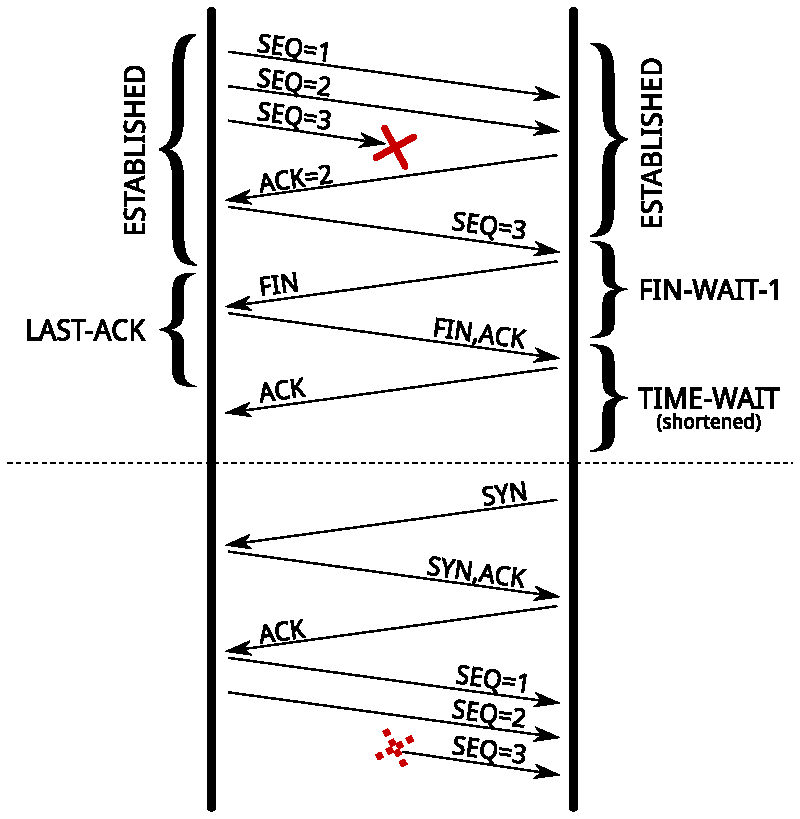
\includegraphics[width=\linewidth]{tcp-dup-seg}
    \end{iblock}
  \end{minipage}\hfill
  \begin{minipage}[b]{.45\linewidth}
    \begin{iblock}{Unexpected RST}
      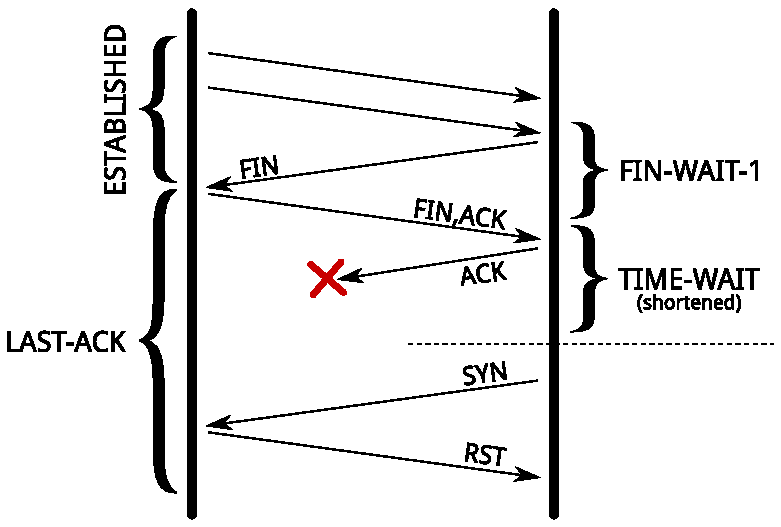
\includegraphics[width=\linewidth]{tcp-last-ack}
    \end{iblock}
  \end{minipage}  
\end{frame}

\begin{frame}{SYN-flood}
  \begin{itemize}
  \item[\$] \cmd{sudo apt install hping3}
  \item[\$] \cmd{sudo tcpdump -ilo port 3333}
  \item[\$] \cmd{ss -anto state syn-recv}
  \item[\$] \cmd{sudo hping3 -\phantom{}-flood -I lo -S -p 3333 127.0.0.1}
  \item[\$] \cmd{sudo iptables -A OUTPUT -p tcp -m tcp -\phantom{}-tcp-flags RST RST -j DROP}
  \item[\$] \cmd{sudo python3 -m http.server 3333}
  % \item[\$] \cmd{sudo iptables -D OUTPUT -p tcp -m tcp --tcp-flags RST RST -j DROP}
  % \item[] 
  % \item[\$] \cmd{\# Syn-flood protection:}
  % \item[\$] \cmd{sudo iptables -A INPUT -p tcp --syn -m limit --limit 1/s -j ACCEPT}
  \end{itemize}
\end{frame}

\begin{itemize}
\item \url{https://www.binarytides.com/tcp-syn-flood-dos-attack-with-hping/}
\item \url{https://linoxide.com/firewall/block-common-attacks-iptables/}
\end{itemize}

%\mode<article>{\clearpage}

\begin{frame}{\texttt{netstat}}
  \CMD{sudo apt install net-tools}
  
  \begin{minipage}[t]{.35\linewidth}
    \begin{itemize}
    \item[\$] \cmd{netstat -ant}
    \item[\$] \cmd{netstat -antp}
    \item[\$] \cmd{netstat -antpe}
    \item[\$] \cmd{netstat -nr}
    \end{itemize}
  \end{minipage}\hfill
  \begin{minipage}[t]{.6\linewidth}
    \begin{itemize}
    \item[\$] \cmd{netstat -ie}
    \item[\$] \cmd{netstat -antp | grep ESTAB}
    \item[\$] \cmd{netstat -nlp | grep :80}
    \item[\$] \cmd{man netstat}
    \end{itemize}
  \end{minipage}
  
  \begin{block}{\texttt{ss} --- a \texttt{netstat} replacement}
    \begin{itemize}
    \item[\$] \cmd{ss -t "( sport = 3333 or dport = 3333 )"}
    \item[\$] \cmd{man ss}
    \end{itemize}
  \end{block}
\end{frame}

\begin{frame}{Sliding Window}
  \begin{center}
    \mode<beamer>{ 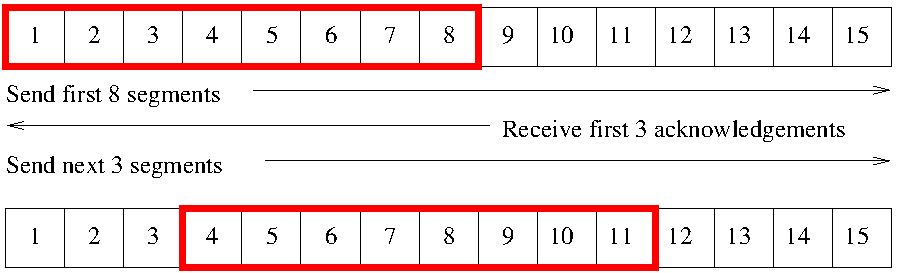
\includegraphics[width=\textwidth]{sliding_window} }%
    \mode<article>{ 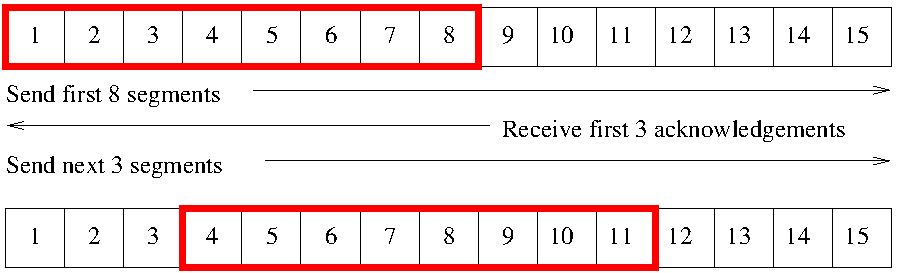
\includegraphics[width=.6\textwidth]{sliding_window} }
  \end{center}
  \begin{iblock}{The sliding window serves several purposes:}
    \begin{itemize}
    \item guarantees the reliable delivery of data
    \item ensures that the data is delivered in order
    \item enforces flow control between the sender and the receiver.
    \end{itemize}
  \end{iblock}
\end{frame}

Flow control vs. congestion control:
\begin{itemize}
\item
  \url{https://stackoverflow.com/questions/16473038/whats-the-difference-between-flow-control-and-congestion-control-in-tcp}
\item
  \url{https://techdifferences.com/difference-between-flow-control-and-congestion-control.html}
\end{itemize}

\begin{frame}<beamer>
  \begin{center}
    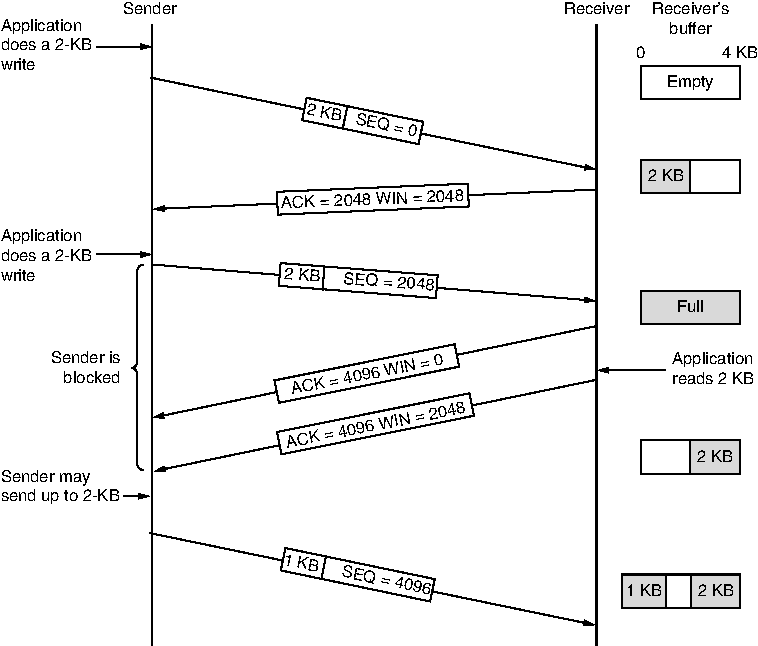
\includegraphics[height=\textheight]{slidingwindow-ast}
  \end{center}
\end{frame}

% \begin{frame}<beamer>
%   \begin{center}
%     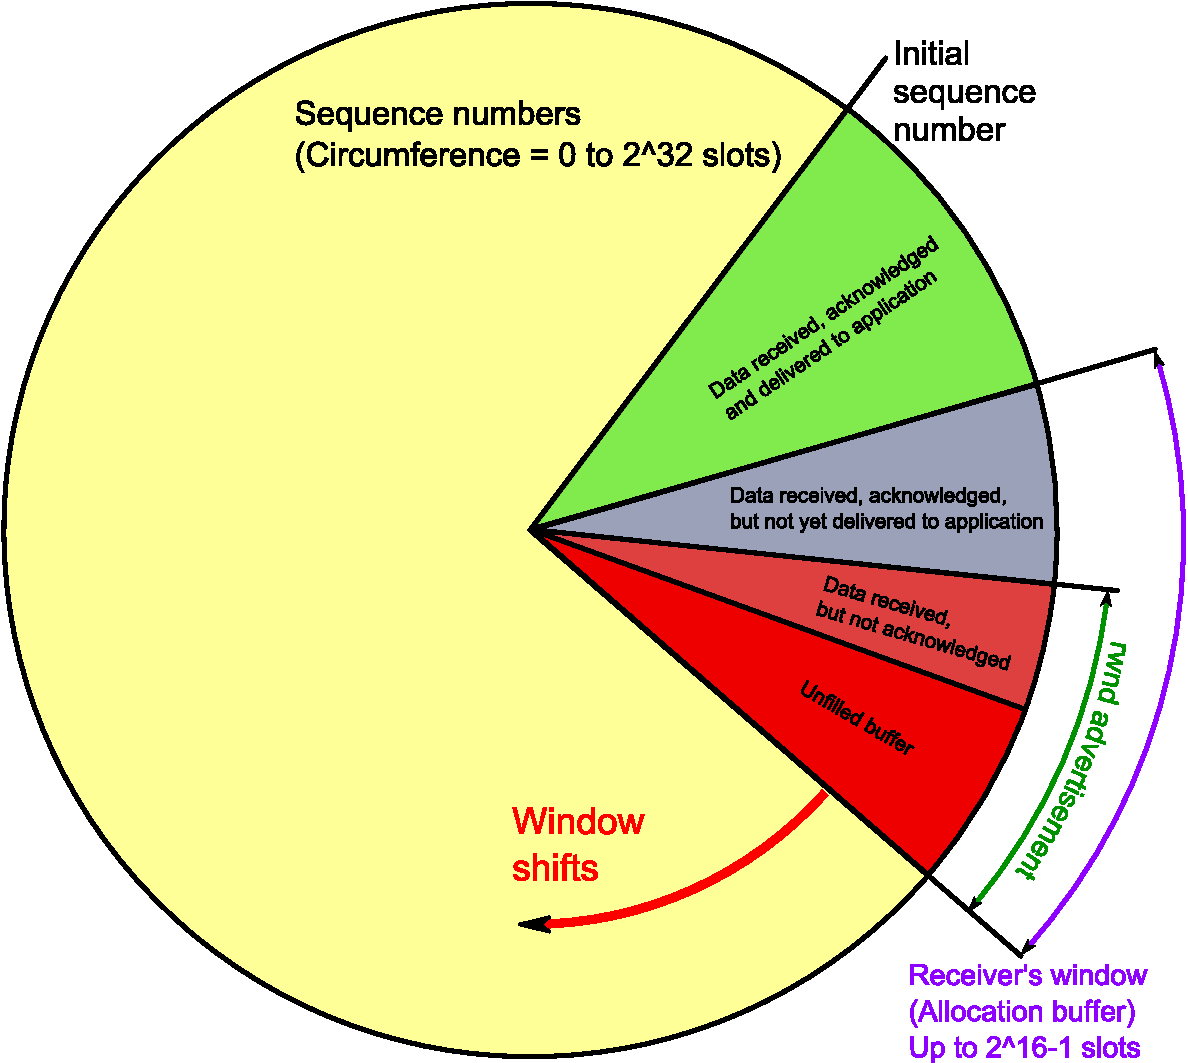
\includegraphics[width=.9\textwidth]{slidingwindow-wiki}
%   \end{center}
% \end{frame}

\begin{minipage}{.48\linewidth}
  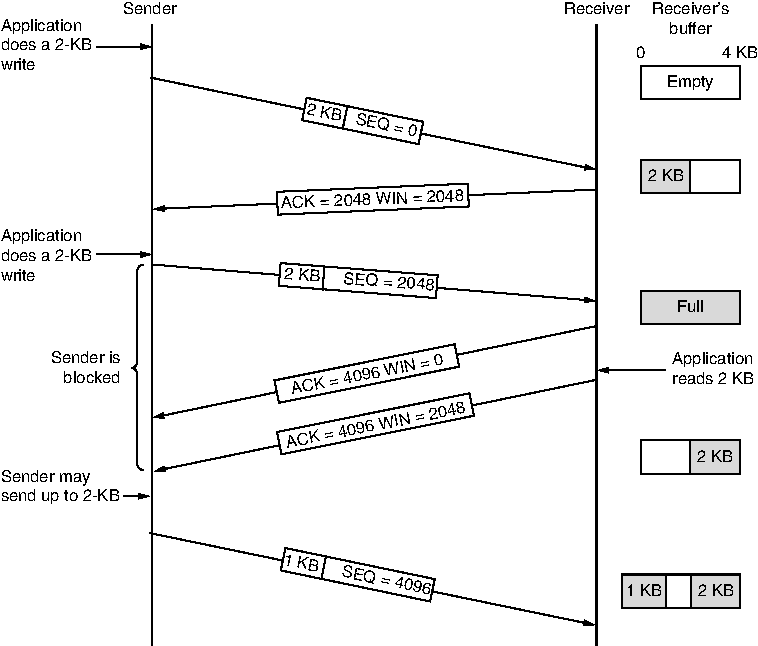
\includegraphics[width=\columnwidth]{slidingwindow-ast}  
\end{minipage}\hfill
\begin{minipage}{.48\linewidth}
  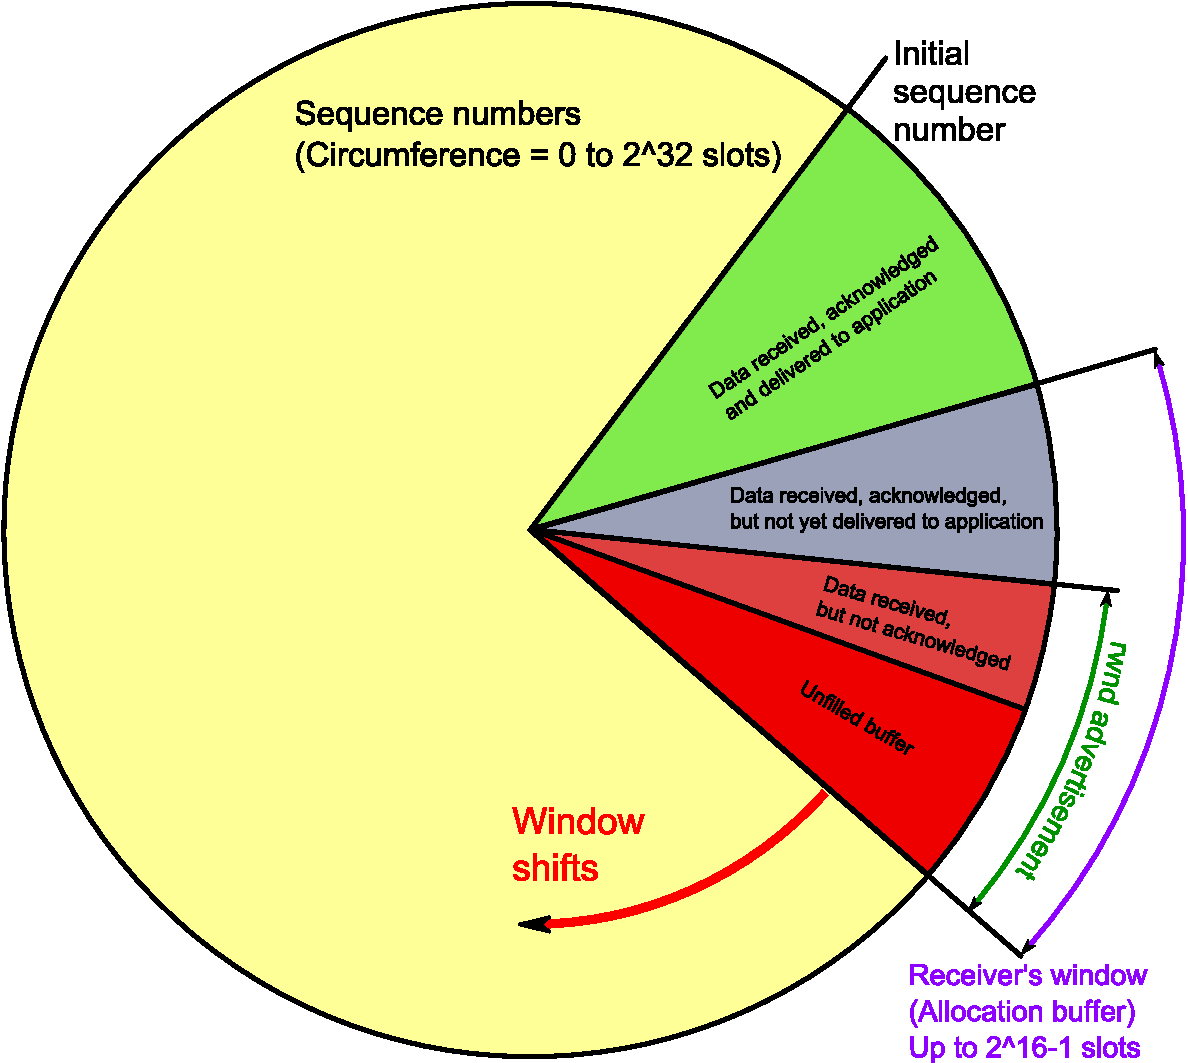
\includegraphics[width=\columnwidth]{slidingwindow-wiki}
\end{minipage}

\begin{frame}
  \begin{minipage}{.4\linewidth}
    \begin{description}
    \item[Packet Lost?] Go-Back-N
    \end{description}
  \end{minipage}\qquad
  \begin{minipage}{.4\linewidth}
    \mode<beamer>{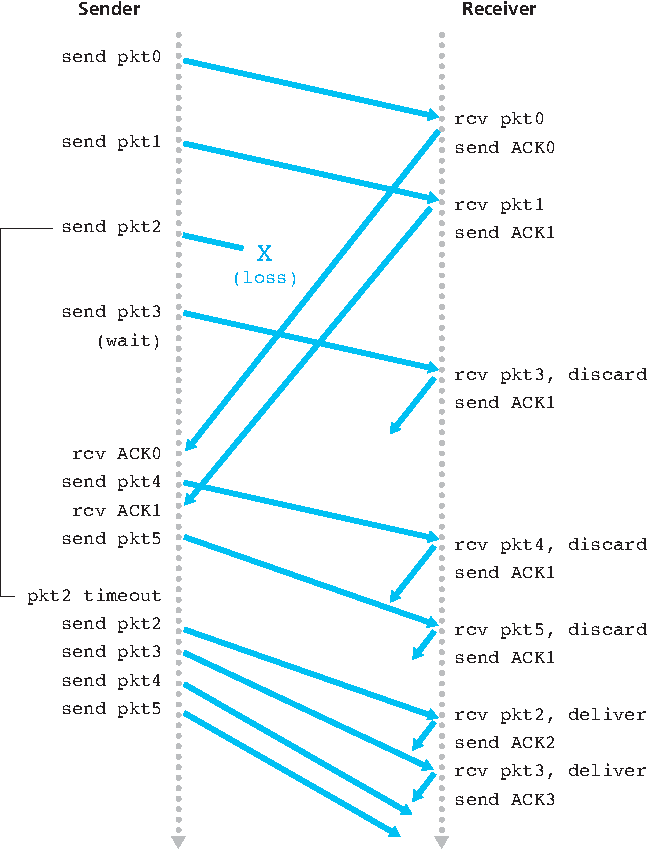
\includegraphics[height=\textheight]{tcp-gbn}}
    \mode<article>{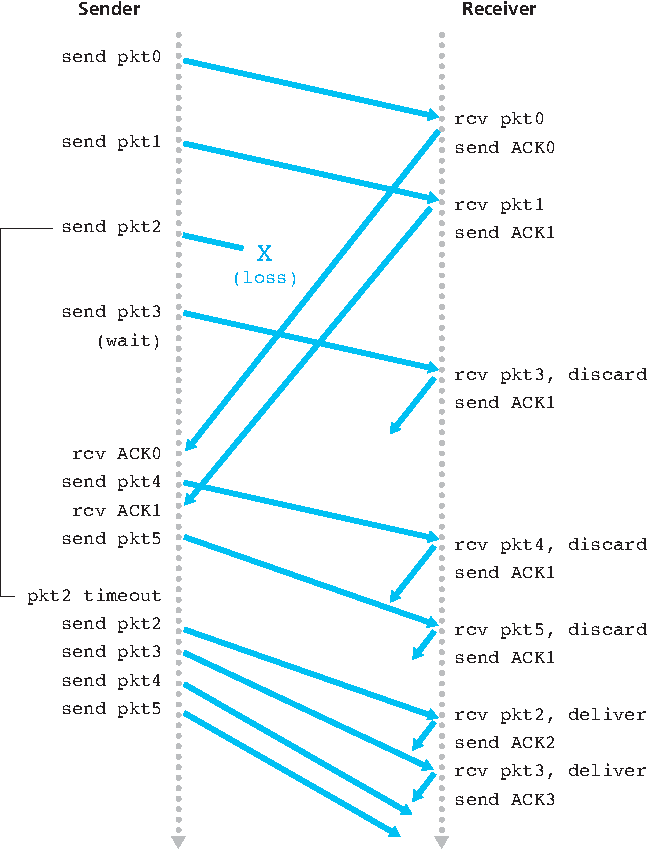
\includegraphics[width=1.5\textwidth]{tcp-gbn}}
  \end{minipage}
\end{frame}

\begin{minipage}{.5\linewidth}
  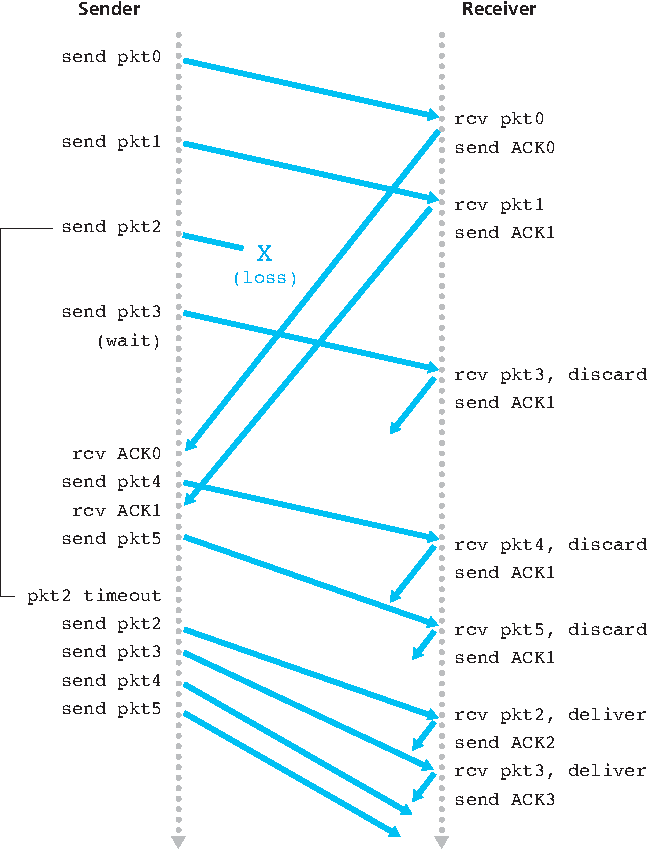
\includegraphics[width=\columnwidth]{tcp-gbn}\label{fig:tcp-gbn}
\end{minipage}\quad
\begin{minipage}{.5\linewidth}
  Figure~\ref{fig:tcp-gbn} shows the operation of the GBN protocol for the case of a
  window size of four packets. Because of this window size limitation, the sender sends
  packets 0 through 3 but then must wait for one or more of these packets to be
  acknowledged before proceeding. As each successive ACK (for example, ACK0 and ACK1) is
  received, the window slides forward and the sender can transmit one new packet (pkt4 and
  pkt5, respectively). On the receiver side, packet 2 is lost and thus packets 3, 4, and 5
  are found to be out of order and are discarded. \citetitle[Sec.~3.4.3, \emph{Go-Back-N
    (GBN)}, P.223]{kurose2013computer}
\end{minipage}

\begin{description}
\item[Cumulative Acknowledgment] \citetitle[Sec.~4.4.1, \emph{Reliable
    Transmission}]{wiki:tcp} TCP primarily uses a cumulative acknowledgment scheme, where
  the receiver sends an acknowledgment signifying that the receiver has received all data
  preceding the acknowledged sequence number. The sender sets the sequence number field to
  the sequence number of the first payload byte in the segment's data field, and the
  receiver sends an acknowledgment specifying the sequence number of the next byte they
  expect to receive. For example, if a sending computer sends a packet containing four
  payload bytes with a sequence number field of 100, then the sequence numbers of the four
  payload bytes are 100, 101, 102 and 103. When this packet arrives at the receiving
  computer, it would send back an acknowledgment number of 104 since that is the sequence
  number of the next byte it expects to receive in the next packet.

  Relying purely on the cumulative acknowledgment scheme employed by the original TCP
  protocol can lead to inefficiencies when packets are lost. For example, suppose 10,000
  bytes are sent in 10 different TCP packets, and the first packet is lost during
  transmission. In a pure cumulative acknowledgment protocol, the receiver cannot say that
  it received bytes 1,000 to 9,999 successfully, but failed to receive the first packet,
  containing bytes 0 to 999. Thus the sender may then have to resend all 10,000
  bytes. \citetitle[Sec.~4.6, \emph{Selective Acknowledgments}]{wiki:tcp}
\end{description}

\begin{frame}<beamer>{ACK lost?}
  \centering
  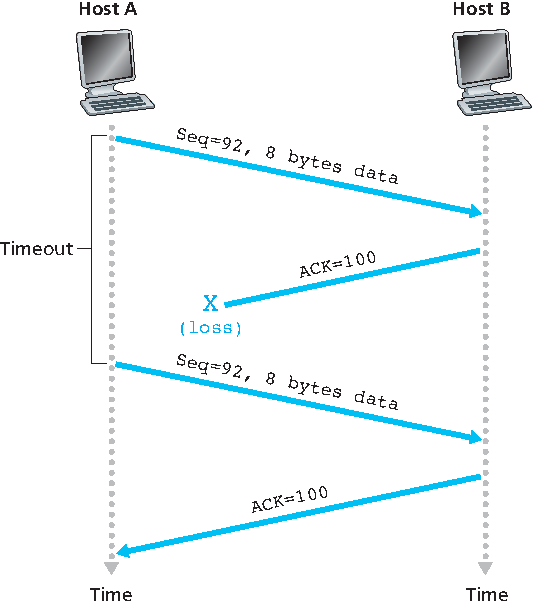
\includegraphics[height=.9\textheight]{tcp-ack-lost}
\end{frame}

\begin{frame}<beamer>[plain]
  \centering
  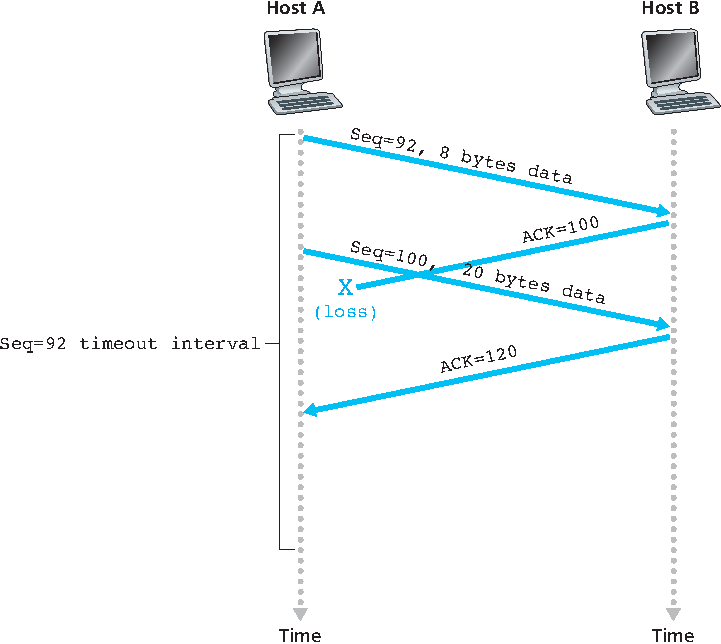
\includegraphics[height=\textheight]{tcp-ack-lost2}
\end{frame}

\begin{minipage}{.42\linewidth}
  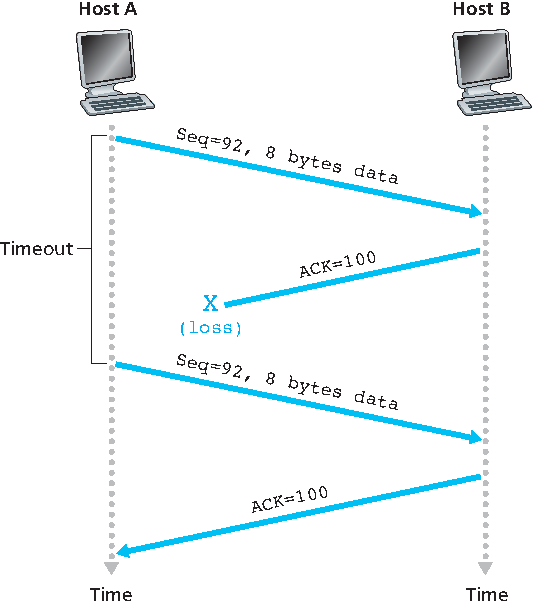
\includegraphics[width=\columnwidth]{tcp-ack-lost}  
\end{minipage}\hfill
\begin{minipage}{.56\linewidth}
  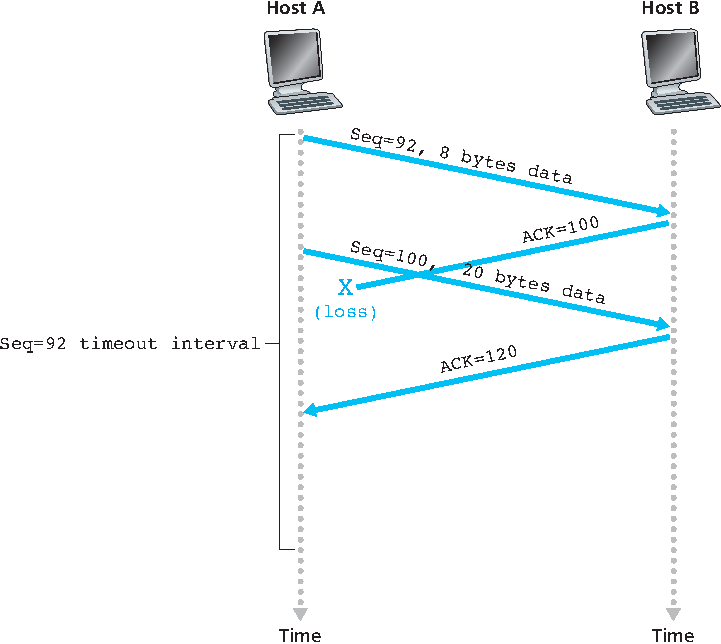
\includegraphics[width=\columnwidth]{tcp-ack-lost2}
\end{minipage}

\begin{frame}{Selective-repeat}
  \centering
  \mode<beamer>{ 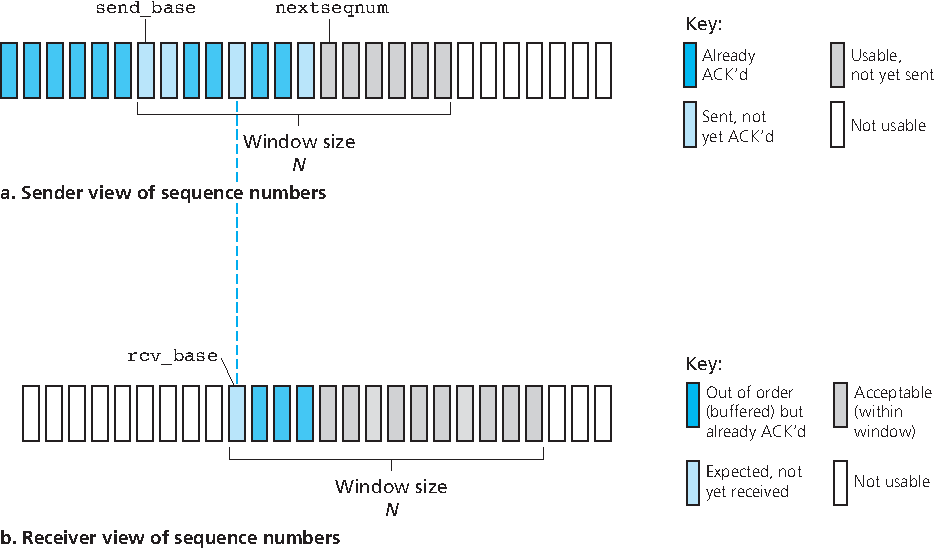
\includegraphics[height=.9\textheight]{tcp-sr} }%
  \mode<article>{ 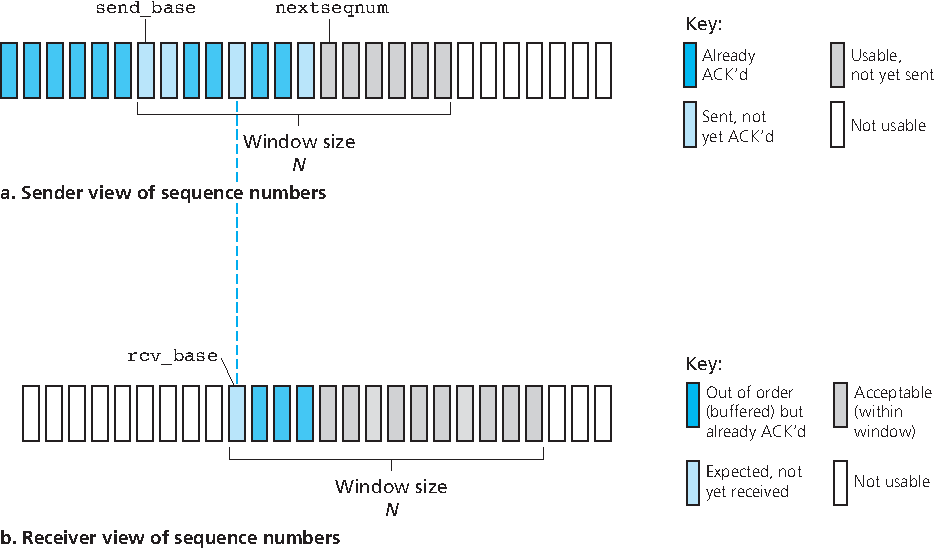
\includegraphics[width=.7\textwidth]{tcp-sr} }
\end{frame}

The SR receiver will acknowledge a correctly received packet whether or not it is in
order. Out-of-order packets are buffered until any missing packets (that is, packets with
lower sequence numbers) are received, at which point a batch of packets can be delivered
in order to the upper layer. \citetitle[Sec.~3.4.4, \emph{Selective Repeat (SR)},
p.~225]{kurose2013computer}

\begin{frame}[plain]
  \begin{center}
    \mode<beamer>{ 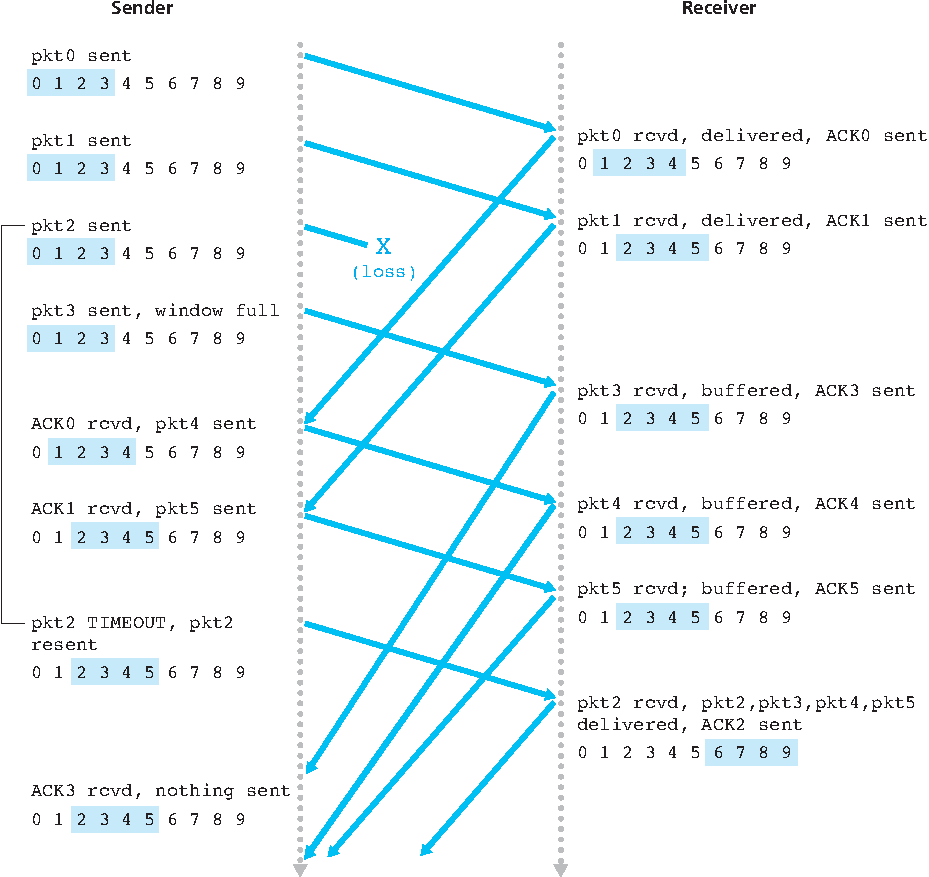
\includegraphics[height=\textheight]{tcp-sr2} }%
    \mode<article>{ 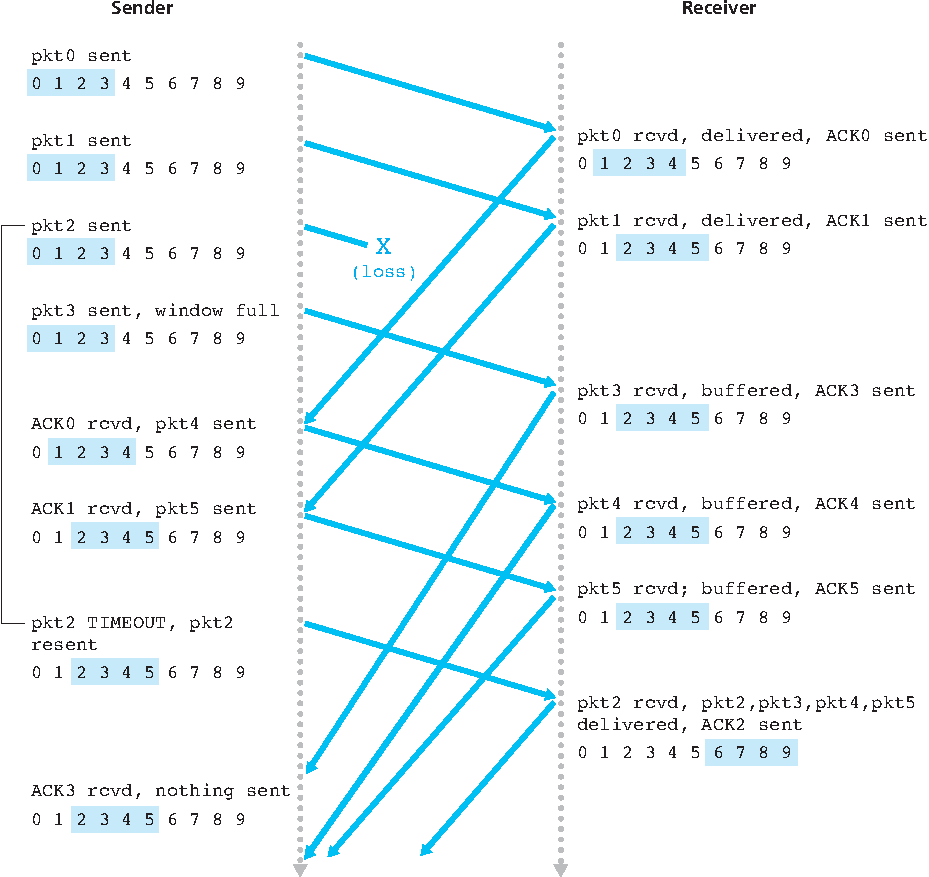
\includegraphics[width=.7\textwidth]{tcp-sr2} }
  \end{center}
\end{frame}

\begin{frame}{TCP Sockets}
  \begin{iblock}{Two Sockets at the Server}
    \centering
    \mode<beamer>{ 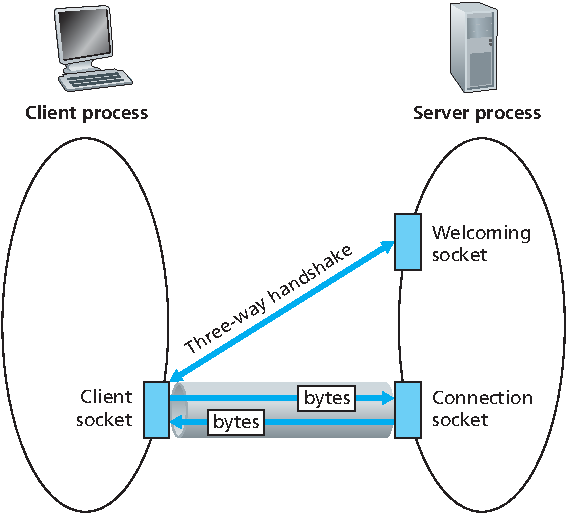
\includegraphics[width=.5\textwidth]{tcpsocket} }%
  \end{iblock}
\end{frame}

\begin{frame}<beamer>%{Stream Sockets}
  \centering
  \mode<beamer>{ 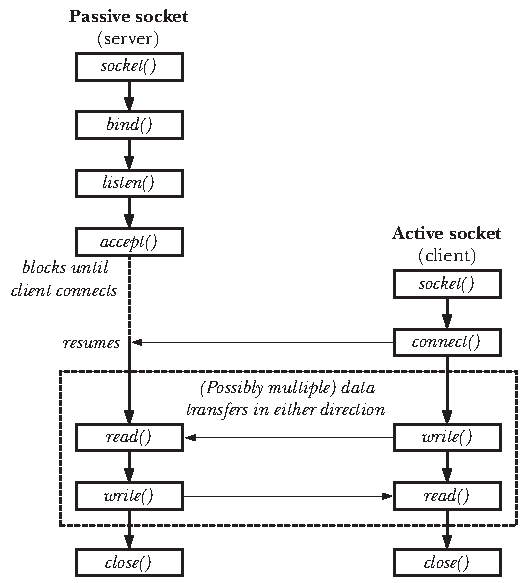
\includegraphics[height=.9\textheight]{socket-stream} }%
\end{frame}

\begin{minipage}{.5\linewidth}
  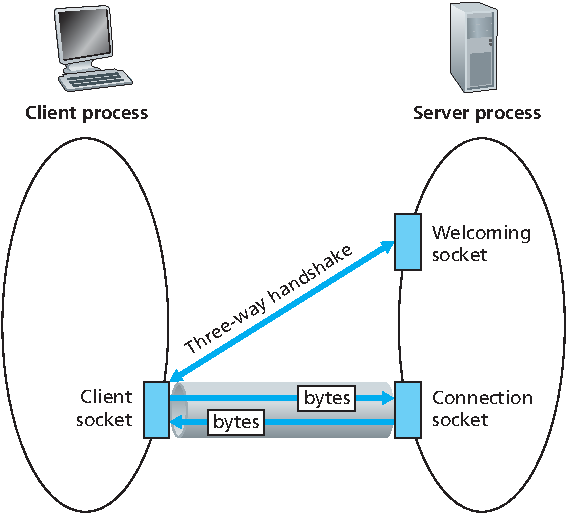
\includegraphics[width=\textwidth]{tcpsocket}
\end{minipage}\hfill
\begin{minipage}{.45\linewidth}
  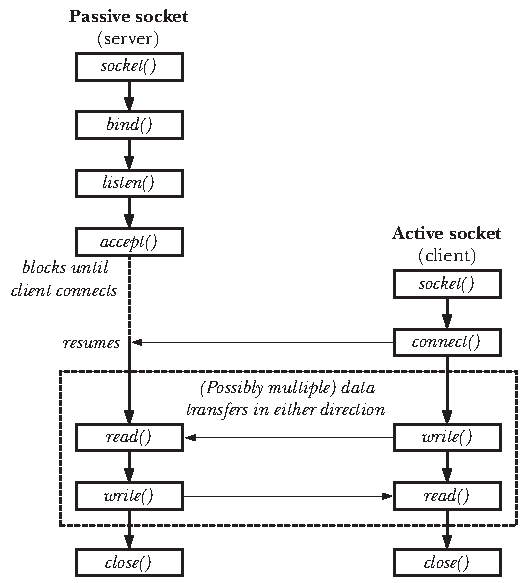
\includegraphics[width=\textwidth]{socket-stream}
\end{minipage}

\begin{frame}{TCPServer.py}
  \begin{minipage}{.5\linewidth}
    \mode<beamer>{ 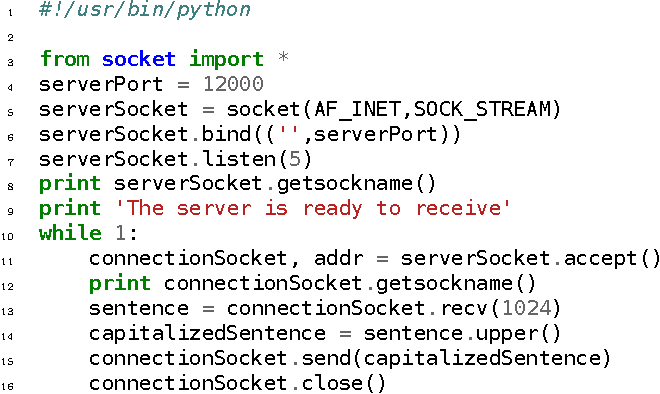
\includegraphics[width=1.2\textwidth]{tcpServer-py} }%
    \mode<article>{ 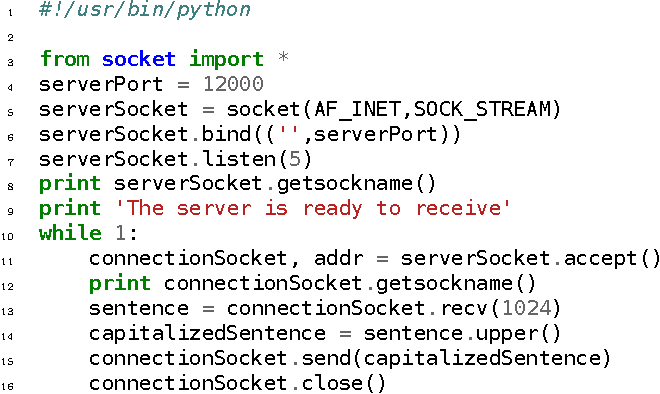
\includegraphics[width=\textwidth]{tcpServer-py} }%
  \end{minipage}\hfill
  \begin{minipage}{.47\linewidth}
    \footnotesize
    \begin{description}
    \item[\texttt{serverSocket}:] the welcoming socket
    \item[\texttt{connectionSocket}:] a socket dedicated to a client
    \item[\texttt{listen(backlog)}:] the server listens for connection requests
      \begin{itemize}\scriptsize
      \item[\texttt{backlog}:] How many non-accepted connection requests
          are allowed to be queueing
      \end{itemize}
    \item[\texttt{accept()}:] whenever a connection request coming, creates a new
      \emph{connectionSocket}
    \end{description}
  \end{minipage}
\end{frame}

\begin{frame}{TCPClient.py}
  \begin{minipage}{.5\linewidth}
    \mode<beamer>{ \includegraphics[width=1.1\textwidth]{tcpClient-py} }%
    \mode<article>{ \includegraphics[width=\textwidth]{tcpClient-py} }%
  \end{minipage}\hfill
  \begin{minipage}{.47\linewidth}
    \begin{description}
    \item[SOCK\_STREAM:] TCP socket
    \item[connect():] initiate the TCP connection (3-way handshake)
    \item[send():] send out \emph{sentence} through the client's socket. No
      destination address needs to be specified
    \end{description}
  \end{minipage}
  \begin{itemize}
  \item[] Re-write it in C or Python3
  \end{itemize}
\end{frame}

\begin{itemize}
\item See also \citetitle[Sec.~3.2, \emph{Multiplexing and
    Demultiplexing}]{kurose2013computer}.
\item The TCP server application has a ``welcoming socket'', that waits for connection
  establishment requests from TCP clients on port number 12000.
\item The TCP client creates a socket and sends a connection establishment request segment
  with the lines:
  \begin{itemize}
  \item[] \cmd{clientSocket = socket(AF\_INET, SOCK\_STREAM)}
  \item[] \cmd{clientSocket.connect((serverName,12000))}
  \end{itemize}
  A connection establishment request is nothing more than a TCP segment with
  destination port number 12000 and a special connection establishment bit (SYN) set in
  the TCP header (discussed in Section 3.5\citetitle{kurose2013computer}). The segment
  also includes a source port number that was chosen by the client.
\item When the host operating system of the computer running the server process receives
  the incoming connection-request segment with destination port 12000, it locates the
  server process that is waiting to accept a connection on port number 12000. The server
  process then creates a new socket:
  \begin{itemize}
  \item[] \cmd{connectionSocket, addr = serverSocket.accept()}
  \end{itemize}
\item Also, the transport layer at the server notes the following four values in the
  connection-request segment: (1) the source port number in the segment, (2) the IP
  address of the source host, (3) the destination port number in the segment, and (4) its
  own IP address. The newly created connection socket is identified by these four values;
  all subsequently arriving segments whose source port, source IP address, destination
  port, and destination IP address match these four values will be demultiplexed to this
  socket. With the TCP connection now in place, the client and server can now send data to
  each other.
\item See also \citetitle[Sec.~2.7, \emph{Socket Programming: Creating Network
    Applications}]{kurose2013computer}.
\end{itemize}

\subsection{UDP}

\begin{frame}{UDP Datagram}
  \begin{center}
    \mode<beamer>{ 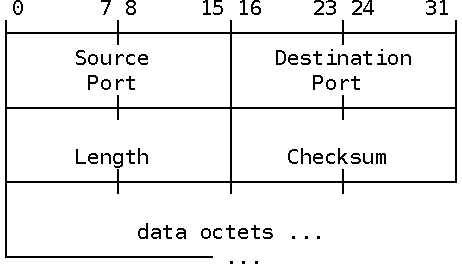
\includegraphics[width=.8\textwidth]{udp-datagram} }%
    \mode<article>{ 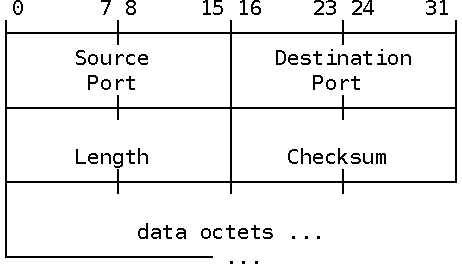
\includegraphics[width=.3\textwidth]{udp-datagram} }
  \end{center}
  \label{fig:udp-datagram-format}
\end{frame}

\begin{frame}{UDP Example}
  \begin{itemize}
  \item[T1:\,\$] \cmd{nc -4ul 3333 \#server}
  \item[T2:\,\$] \cmd{nc -4u localhost 3333 \#client}, or
  \item[\$] \cmd{echo hello > /dev/udp/127.0.0.1/3333}
  \item[T3:\,\$] \cmd{sudo tcpdump -ilo udp port 3333}
  \item[T4:\,\$] \cmd{watch -tn.1 \textbackslash}
  \item[>] \cmd{'ss -4au "( sport = 3333 or dport = 3333 )"'}
  \end{itemize}
\end{frame}

\begin{description}
\item[Why need checksum?]  See also \citetitle[Sec.~3.3.2, \emph{UDP
    Checksum}]{kurose2013computer}.
  \begin{enumerate}
  \item (layer 2) there is no guarantee that all the links between source and destination
    provide error checking;
  \item (layer 3) even if segments are correctly transferred across a link, it's possible
    that bit errors could be introduced when a segment is stored in a router's memory.
  \end{enumerate}
\end{description}

\begin{frame}{Datagram Sockets}
  \centering%
  \mode<beamer>{ 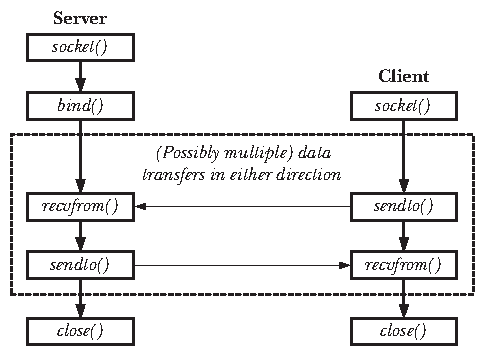
\includegraphics[width=.7\textwidth]{socket-datagram} }%
  \mode<article>{ 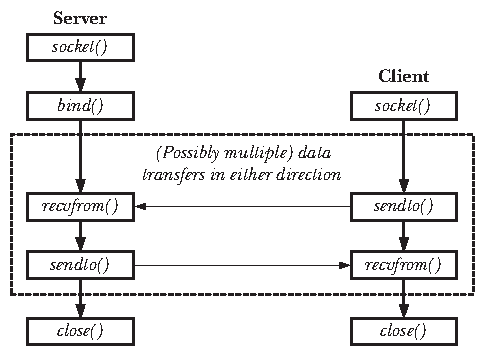
\includegraphics[width=.6\textwidth]{socket-datagram} }
\end{frame}

\begin{frame}{UDPServer.py}
  \begin{center}
    \mode<beamer>{ \includegraphics[width=\textwidth]{udpServer-py} }%
    \mode<article>{ \includegraphics[width=.5\textwidth]{udpServer-py} }
  \end{center}
  \begin{iblock}{\texttt{serverSocket.bind(('\,', serverPort))}}
    \begin{itemize}
    \item explicitly assigns \texttt{12000} to the server's socket
    \end{itemize}
  \end{iblock}
\end{frame}

\begin{frame}[t,allowframebreaks]{UDPClient.py}
  \begin{center}
    \mode<beamer>{ 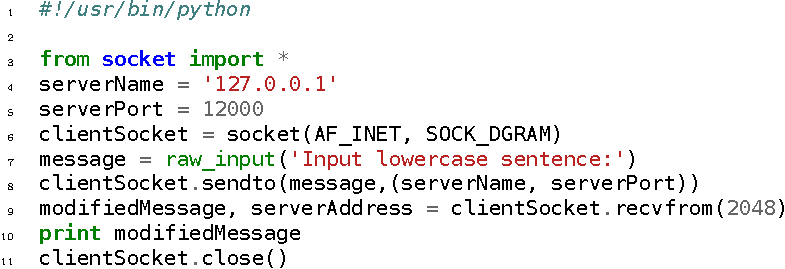
\includegraphics[width=\textwidth]{udpClient-py} }%
    \mode<article>{ 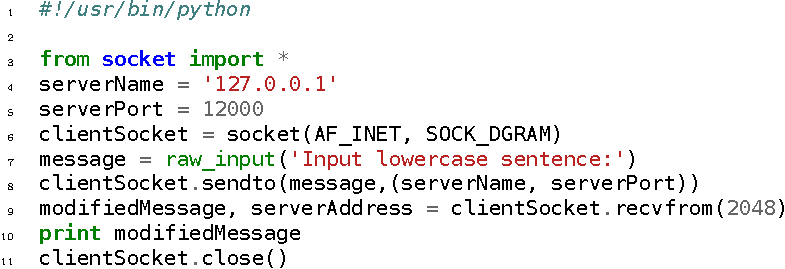
\includegraphics[width=.5\textwidth]{udpClient-py} }
  \end{center}
  \begin{iblock}{\texttt{socket(AF\_INET, SOCK\_DGRAM)}}
    \begin{itemize}
    \item \texttt{AF\_INET}: using IPv4
    \item \texttt{SOCK\_DGRAM}: UDP socket
    \item \texttt{clientPort} will be generated automatically
    \end{itemize}
  \end{iblock}
  \begin{iblock}{\texttt{clientSocket.sendto(message,(serverName, serverPort))}}
    \begin{enumerate}
    \item attaches both the destination address \texttt{(serverName, serverPort)} and the
      source address \texttt{(clientIP, clientPort)} to the message
    \item send the message
    \end{enumerate}
  \end{iblock}
  \begin{iblock}{\texttt{modifiedMessage, serverAddress = clientSocket.recvfrom(2048)}}
    \begin{enumerate}
    \item puts the received message data into \texttt{modifiedMessage}
    \item puts the source address \texttt{(IP, Port)} into \texttt{serverAddress}
    \end{enumerate}
    \begin{itemize}
    \item \texttt{2048}: buffer size
    \end{itemize}
  \end{iblock}
\end{frame}

\begin{frame}{TCP/UDP References}
  \begin{refsection}
    \nocite{wiki:tcp, wiki:udp, wiki:checksum, rfc793, rfc768, wiki:socket, hall2009beej}
    \printbibliography[heading=none]
  \end{refsection}
\end{frame}

\mode<all>
%%% Local Variables:
%%% mode: latex
%%% TeX-master: "net-b"
%%% End:
